\documentclass[parskip=half, titlepage=firstiscover, captions=tableheading, bibliography=totoc]{scrartcl}
%optionen immer variieren tabelheading bei tabellen
%ohne parskip nur einrücken
%draft macht hüllen von bilder selbst wenn sie nicht existieren um einfach zeit bei compilieren zu sparen
%\usepackage{scrhack} % nach \documentclass
\usepackage{float}
\floatplacement{figure}{htbp}
\floatplacement{table}{htbp}
\usepackage[aux]{rerunfilecheck}
\usepackage{polyglossia}
\usepackage{biblatex}
\addbibresource{Tag3.bib}%name der bib-Datei hier einfügen !
\setmainlanguage{german}
\usepackage{longtable}
\usepackage{amsmath}
\usepackage{amssymb}
\usepackage{mathtools}
\usepackage{fontspec}
\usepackage[
math-style=ISO,
bold-style=ISO,
sans-style=italic,
nabla=upright,
partial=upright,
]{unicode-math}

\setmathfont{Latin Modern Math}
\usepackage{graphicx}
\usepackage{grffile}
\usepackage[font = scriptsize, labelfont = bf,margin={10pt,10pt}]{subcaption}
\usepackage[font = scriptsize, labelfont = bf,margin={10pt,10pt}]{caption}
%anstatt margin geht auch width = 10cm
\usepackage{mleftright}
%schöneres mit  \mleft (\mright)

\setlength{\delimitershortfall}{-1sp}
%bei vielen Klammern werden sie nun größer
\usepackage[locale=DE,separate-uncertainty=true,per-mode=symbol-or-fraction]{siunitx}
\usepackage{booktabs}
\usepackage{xfrac}
\usepackage{pdflscape}
%-> dazu wäre begin{landscape} etc nötig

%nur ein beispiel zu dieser änderung wenn man will
%gleiche sachen werden bei mathe oder text anders benutzt
%\let\vaccent=\v % alten Befehl kopieren
%\RenewDocumentCommand \v {} % Befehl überschreiben
%{
%\TextOrMath{
%\vaccent % Textmodus
%}{
%\symbf % Mathemodus
%}
%}

%\NewDocumentCommand \OverfullCenter {+m} {
%\noindent\makebox[\linewidth]{#1} }
%bei zu breiten pics zentrierte ausrichtung
%zu befehl wäre dann: \OverfullCenter{\includegraphics[width=\textwidth+15pt]{figures/
%Panorama.jpg}}

\AtBeginDocument{ % wird bei \begin{document} ausgeführt
\let\symIm=\Im % werden sonst wieder von unicode-math überschrieben
\RenewDocumentCommand \Re {}
{
\operatorname{Re}
}
\let\symIm=\Im
\RenewDocumentCommand \Im {}
{
\operatorname{Im}
}
}


\usepackage{fontspec}%nach amssymb
\usepackage[unicode]{hyperref}
\usepackage[shortcuts]{extdash} % nach hyperref, bookmark am Ende!
\usepackage{bookmark}

\usepackage[locale=DE,separate-uncertainty=true,per-mode=symbol-or-fraction]{siunitx}


\begin{document}
\section{Auswertung}
\label{sec:Auswertung}
Hier folgt nun die Auswertung des Experiments, das mit Hilfe des Gräts $2$ durchgeführt wurde.
Die Plots wurden mit Hilfe des Programs Gnuplot erstellt.
\subsection[underline]{Zeitabhängigkeit der gedämpften Schwinungsamplitude}
Zuerst wurde die abklingenden Amplituden $U_C$ mit dem Fehler $\pm{0,08}$$\si{\volt}$ des LCR-Schwingkreises im Bezug auf
die Zeit $t_i$ mit der Ungenauigkeit von $\pm{2}$$\si{\micro\s}$ gemessen.(Siehe Abbildung \ref{fig:thermodruck})
\begin{table}
  \centering
  \caption{Hier sieht man deutlich den exponentiellen Abfall der Ampiltuden der Schwingung mit $\SI{1997}{\hertz}$ Eregerfrequenz zu der Zeit}
  \label{tab:Daten1}
  \begin{tabular}{S S}
   \toprule
   {$U_C\:/\:\si{\volt}$} & {$t_i\:/\:\si{\micro\sec}$} \\
   \midrule
  4,56 & 12\\
  3,76 & 28\\
  3,36 & 44\\
  2,64 & 56\\
  2,40 & 70\\
  2,24 & 86\\
  1,76 & 102\\
  1,60 & 116\\
  1,36 & 128\\
  1,20 & 146\\
  0,96 & 158\\
  0,96 & 173\\
  0,80 & 186\\
  0,72 & 202\\
  0,56 & 216\\
  0,56 & 230\\
  0,48 & 240\\
   \bottomrule
  \end{tabular}
 \end{table}
Besonders hervor zu heben ist der Dämpfungswiderstand des aperiodischen Grenzfalls,der experimentel einen Wert von $\SI{3,19(1)}{\kilo\ohm}$ beträgt.
Verglichen mit dem durch () errechneten Widerstand von $\SI{4,39(9)}{\kilo\ohm}$, ist eine Differenz von ~ $\SI{1,4}{\kilo\ohm}$ zu ersehen.
Durch die Ausgleichrechnung () erhält man $\mu$ aus dem Exponenten der Gleichung () und kann somit folgendes berechnen:
\begin{align*}
 T_{ex} &= \si{123(1)e-6}{\sec}\\
 R_{eff} &= \SI{123(1)}{\ohm}
\end{align*}
Vergleicht man nun den effektiven Widerstand $R_{eff}$ mit dem in der Schaltung eingesetzten von $\SI{48,1(1)}{\ohm}$ , ist eine Diskrepanz von ungefähr $\SI{50}{\ohm}$ zu erkennen.
\begin{figure}
\centering
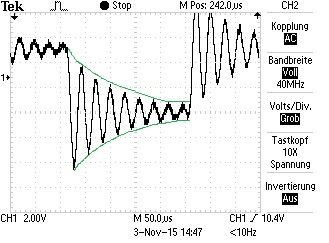
\includegraphics{Thermo.jpg}
\caption{Thermodruck des zeitlichen Abklingens der gedämpften Schwingungsamplitude\\ mit der Einfüllenden(in grün).}
\label{fig:thermodruck}
\end{figure}
\newpage
\subsection[underline]{Messung der Frequenzabhängigkeiten an einem LCR-Schwingkreis}
In der folgenden Tabelle sind die Daten aus der Messreihe der Kondensatorspannung  mit der Ungenauigkeit $\pm{0,3}$$\si{\volt}$ zu den Frequenzenmit mit der Ungenauigkeit $\pm{0,03}$$\si{\kilo\hertz}$, sowie das Verhältnis dieser zur Eregerspannung von ca. $\SI{10}{\volt}$ zu finden.
Diese Daten sind in zwei Plots einem in linearel (\ref{fig:Linear1}) und einem in halblogarithmischer (\ref{fig:Halb1}) Form aufgetragen.
Wichtig hierbei zu erwähnen ist,dass ab einschließlich dem Wert $\SI{27,15}{\kilo\hertz}$ die Skala vergrößert wurde, sodass sich die darauffolgenden Werte leicht verschieben können.
Aus dem Linearen der darauffolgenden Plots, in dem die Frequenz zum Spannungsverhältnis aufgetragen wurde, sind die experimentellen Werte für die Resonanzüberhöhung bzw. Güte q, sowie die Breite der Resonanzkurve $\nu_1 - \nu_2$ entnommem und werden hier mit den durch () berechneten Werten mit einem Gesamtwiderstand von $\SI{559,5(5)}{\ohm}$ verglichen:
\begin{align*}
q_{theo} &= \si{3,923(5)} & q_{exp} &= \si{3,72}\\
\text{Theoretisch:} \symup{\nu_+} - \symup{\nu_-} &= \SI{8,81(3)e3}{\hertz} & \text{Experimentell:} \symup{\nu_+} - \symup{\nu_-} &= \SI{11,19e3}{\hertz}
\end{align*}
Die realtiv gerringen Differnezen von q bei etwa $0,2$ und bei Resonanzkurvenbreite bei etwa $\SI{1,3e3}{\ohm}$ sind im Fehlertolerenazbereich und benötigen somit keine weitere Erläuterung.
\begin{table}
  \centering
  \caption{Die Messdaten zeigen hierbei einen deutlichen Anstieg bis zum Maximum, sowie eine nachträglichen Abfall gleichermaßen}
  \label{tab:Daten2}
  \begin{tabular}{S S S}
    \toprule
    \multicolumn{1}{c}{$\si{\nu}\:/\:\si{\kilo\hertz}$} & \multicolumn{1}{c}{$U_C\:/\:\si{\volt}$} & \multicolumn{1}{c}{$U_C/U$}\\
    \midrule
    2,00 & 10,0 & 1,00\\
    4,00 & 10,0 & 1,00\\
    5,00 & 10,2 & 1,02\\
    7,50 & 10,4 & 1,04\\
    9,00 & 10,6 & 1,06\\
   11,00 & 11,0 & 1,10\\
   14,00 & 11,5 & 1,15\\
   16,00 & 12,0 & 1,20\\
   18,00 & 12,6 & 1,26\\
   18,65 & 13,0 & 1,30\\
   19,50 & 13,6 & 1,36\\
   20,30 & 14,0 & 1,40\\
   21,00 & 14,6 & 1,46\\
   21,45 & 15,0 & 1,50\\
   22,50 & 15,8 & 1,58\\
   23,00 & 16,3 & 1,63\\
   23,60 & 16,9 & 1,69\\
   24,20 & 17,6 & 1,76\\
   24,55 & 18,0 & 1,80\\
   25,00 & 18,6 & 1,86\\
   25,35 & 19,0 & 1,90\\
   25,65 & 19,4 & 1,94\\
   26,10 & 20,1 & 2,01\\
   26,50 & 20,7 & 2,07\\
   26,80 & 21,2 & 2,12\\
   27,10 & 21,7 & 2,17\\
   27,15 & 22,4 & 2,24\\
   27,50 & 22,8 & 2,28\\
   28,00 & 24,0 & 2,40\\
   28,40 & 24,8 & 2,48\\
   28,60 & 25,2 & 2,52\\
   29,05 & 26,4 & 2,64\\
   29,35 & 27,2 & 2,72\\
   29,50 & 27,6 & 2,76\\
   29,85 & 28,4 & 2,84\\
   30,00 & 28,8 & 2,88\\
   30,15 & 29,2 & 2,92\\
   30,25 & 29,6 & 2,96\\
   30,45 & 30,0 & 3,00\\
   30,55 & 30,4 & 3,04\\
   30,70 & 30,8 & 3,08\\
   30,85 & 31,2 & 3,12\\
   31,00 & 31,6 & 3,16\\
   31,10 & 32,0 & 3,20\\
   31,25 & 32,4 & 3,24\\
   31,55 & 33,4 & 3,34\\
   31,70 & 33,2 & 3,32\\
   31,90 & 34,0 & 3,40\\
   32,20 & 34,8 & 3,48\\
   32,35 & 35,2 & 3,52\\
   32,55 & 35,6 & 3,56\\
   32,80 & 36,0 & 3,60\\
   33,35 & 36,8 & 3,68\\
   34,00 & 37,2 & 3,72\\
   34,50 & 36,8 & 3,68\\
   35,00 & 36,4 & 3,64\\
   35,50 & 35,2 & 3,52\\
   36,00 & 33,6 & 3,36\\
   36,50 & 32,3 & 3,23\\
   37,00 & 30,6 & 3,06\\
   37,50 & 29,0 & 2,90\\
   38,00 & 27,2 & 2,72\\
   38,50 & 25,6 & 2,56\\
   39,00 & 24,0 & 2,40\\
   39,50 & 22,4 & 2,24\\
   40,00 & 21,2 & 2,12\\
   41,00 & 19,0 & 1,90\\
   42,00 & 16,8 & 1,68\\
   43,00 & 15,2 & 1,52\\
   44,00 & 14,0 & 1,40\\
   45,00 & 12,8 & 1,28\\
   46,00 & 11,6 & 1,16\\
   47,00 & 10,8 & 1,08\\
   48,00 & 10,0 & 1,00\\
   49,00 & 9,2 & 0,92\\
   50,00 & 8,6 & 0,86\\
   55,00 & 6,4 & 0,64\\
\bottomrule
\end{tabular}
\end{table}
\begin{figure}
  \centering
  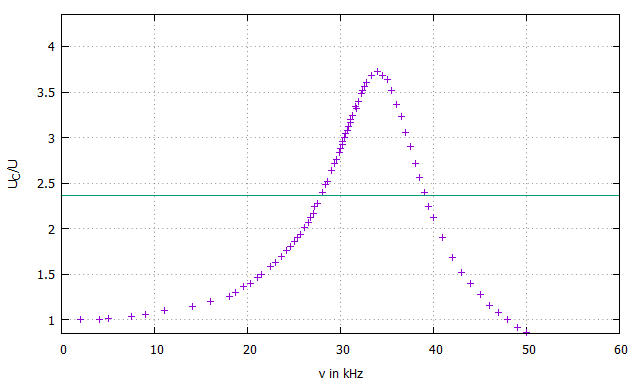
\includegraphics[width=\textwidth]{Linear1.jpeg}
\caption{Aus der hierzusehenden linearen Darstellung der Freuquenzabhänigkeit der Spannung \\ sind die Daten zur Güte und die Resonanzkurve mit ihren eingezeichten Ränder anzulesen.}
\label{fig:Linear1}
\end{figure}
\begin{figure}
  \centering
  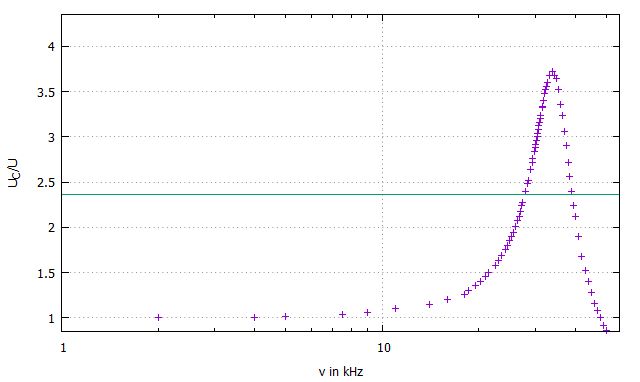
\includegraphics[width=\textwidth]{Halblog1.jpeg}
  \caption{Hier ist die halblogarithmische Darstellung des Spannungs-Frequenzverhältnisses zu sehen.}
  \label{fig:Halb1}
\end{figure}

\subsection[underline]{Messung der Phasen zwischen Erreger- und Kondensatorspannung}
Im letzten Teil des Experiments wurden die Phasendifferenzen $\delta$t zu den einzelnen Frquenzen gemessen und daraus die Pahsenverschiebuung $\varphi$ im Bogenmaß berechnet.
Hier sind die Phasenverschiebung $\varphi$ und die Phasendifferenz $\delta$t mit der Ungenauigkeit $\pm{0,2}$$\si{\micro\s}$ zur Frequenz $\nu$ vom Verhälnis LCR-Schwingkreis zu Sinus-Schwingungsgenerator.
\begin{table}
  \centering
  \caption{Hier sieht man die Werte, der durch Lissajou-Figuren gemessenen Phasendifferenz, und die dazugehörige Verschiebung zu den Frequenzen.}
  \label{tab:Daten3}
  \begin{tabular}{S S S}
    \toprule
    \multicolumn{1}{c}{$\symup{\nu}\:/\:\si{\kilo\hertz}$} & \multicolumn{1}{c}{$\symup{\Delta}t\:/\:\si{\micro\sec}$} & \multicolumn{1}{c}{$\symup{\varphi}\:/\:rad$}\\
    \midrule
    2,0 & 0,00 & 0,0000 \\
    5,0 & 1,00 & 0,0314 \\
   10,0 & 1,00 & 0,0628 \\
   15,0 & 1,50 & 0,1414 \\
   20,0 & 1,80 & 0,2262 \\
   25,0 & 2,10 & 0,3300 \\
   27,5 & 3,00 & 0,5184 \\
   30,0 & 4,00 & 0,7540 \\
   30,5 & 4,10 & 0,7854 \\
   31,0 & 4,50 & 0,8765 \\
   32,0 & 5,20 & 1,0455 \\
   33,0 & 6,00 & 1,2440 \\
   33,5 & 6,50 & 1,3681 \\
   34,0 & 6,70 & 1,4313 \\
   34,5 & 7,50 & 1,6258 \\
   35,0 & 7,50 & 1,6493 \\
   35,5 & 8,00 & 1,7844 \\
   36,0 & 8,50 & 1,9227 \\
   36,5 & 8,70 & 1,9952 \\
   37,0 & 9,00 & 2,0923 \\
   37,5 & 9,25 & 2,1795 \\
   38,0 & 9,50 & 2,2682 \\
   38,5 & 9,50 & 2,2980 \\
   39,0 & 9,50 & 2,3279 \\
   39,5 & 9,75 & 2,4198 \\
   40,0 & 9,75 & 2,4504 \\
   \bottomrule
 \end{tabular}
 \end{table}

Die Plots der Frequenzen in Abhängigkeit der Phasenverschiebung sind in halblogarithmischer (\ref{fig:Halb2}) und linearer (\ref{fig:Linear2}) Form in den folgenden Abbildungen zusehen.\\
Aus Letztrem werden die experimentellen Werte für die Resonanzspannung $\nu_res$ , die sich im Bereich von $\pi/2$ befindet, sowie die Ränder der Resonanzkurve $\nu_1$ und $\nu_2$ bei $\pi/4$ und $3*\pi/2$ entnommen.
\begin{figure}
  \centering
  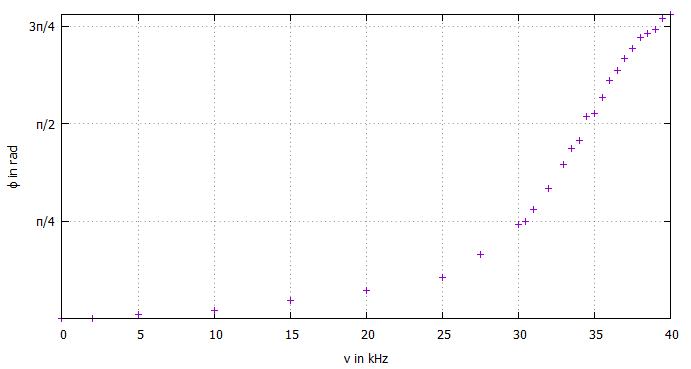
\includegraphics[width=\textwidth]{Linear2.jpeg}
  \caption{Die lineare Darstellung des Verhältnisses Phasenverschiebung von Erreger- und Kondensatorspannung zur Frequenz.}
  \label{fig:Linear2}
\end{figure}
Hier in der linearen Abbildung ist gut der extreme Antsieg der arctan-annäherden Kurve zu sehen.\\Die Spitze und ihr Abflachen sind, durch die begrentzte Maximalfrequenz nur zu erahnen.
\begin{figure}
  \centering
  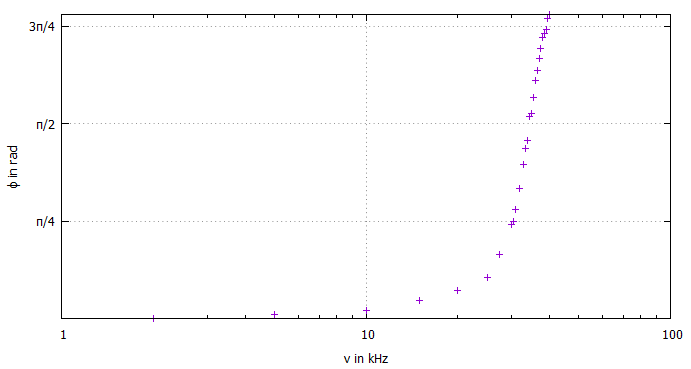
\includegraphics[width=\textwidth]{Halblog2.jpeg}
  \caption{Die halblogarithmische Darstellung der Ferquenzabhängigkeit der Phase zwischen Erreger- und Kondensatorspannung.}
  \label{fig:Halb2}
\end{figure}
\newpage
Die experimentellen Werte werden mit den durch () und () berechneten Werten verglichen:
\begin{align*}
  \text{Theoretisch:}\nu_{res} &= \SI{34,55(8)}{\kilo\hertz} & \nu_1 &= \SI{30,78(4)}{\kilo\hertz} & \nu_2 &= \SI{38,80(3)}{\kilo\hertz}\\
  \text{Experimentell:}\nu_{res} &= \SI{34,60}{\kilo\hertz} & \nu_1 &= \SI{30,50}{\kilo\hertz} & \nu_2 &= \SI{39,0}{\kilo\hertz}
\end{align*}
 \end{document}
